%\VignetteIndexEntry{Introduction to SpaDES: A package to develop and run spatially explicit discrete event simulation models.}
%\VignetteDepends{SpaDES}
%\VignetteKeyword{discrete event simulation}
\documentclass{article}

%%% latex packages
\usepackage[T1]{fontenc}
\usepackage{hyperref}
\usepackage[utf8]{inputenc}
\usepackage[usenames,dvipsnames]{xcolor}

%% change margins to 1" all the way around
\oddsidemargin 0.0in
\evensidemargin 0.0in
\textwidth 6.5in
\headheight 0.0in
\topmargin 0.0in
\textheight 9.0in

%%% document info
\title{Introduction to \texttt{SpaDES}}

\author{
  Alex M. Chubaty\\
	\small{Natural Resources Canada, Pacific Forestry Centre}\\
	\small{email: \href{mailto:achubaty@nrcan.gc.ca}{achubaty@nrcan.gc.ca}}
	\and
	Eliot McIntire\\
	\small{Natural Resources Canada, Pacific Forestry Centre}\\
	\small{email: \href{mailto:emcintir@nrcan.gc.ca}{emcintir@nrcan.gc.ca}}
}

\usepackage{Sweave}
\begin{document}
\Sconcordance{concordance:introduction.tex:introduction.Rnw:%
1 31 1 1 0 14 1 1 3 2 0 1 1 1 10 8 0 1 2 7 0 1 5 14 1 1 2 1 0 4 1 1 2 4 %
0 1 2 22 1 1 2 1 0 1 4 2 0 1 2 1 0 3 1 1 5 3 0 1 1 1 2 11 0 1 1 15 0 1 %
7 5 0 1 2 5 0 1 2 7 1}

 % displays code as entered (no arranging lines)

\maketitle

\abstract{Implement a variety of simulation models, with a focus on spatially explicit raster models and agent based models. The core simulation components are built upon a discrete event simulation framework that facilitates modularity, and enables the user to include additional functionality by running user-built simulation modules. Included are numerous tools to visualize raster and other maps.\\
\\
\textbf{Website:} \url{https://github.com/achubaty/SpaDES}}

\tableofcontents

\newpage

\section{Introduction}

\subsection{Objectives and motivations}

\paragraph{}
Building spatial simulation models often involves reusing various components, often having to reimplement similar fuctionality in multiple simulation frameworks (i.e, in different programming languages). When various components of a simulaiton model become fragmented across multiple platforms, it becomes increasingly difficult to link these various components, and often solutions for this problem are idiosyncratic and specfic to the model being implemented.

\paragraph{}
\texttt{SpaDES} is a generic simulation platform that can be used to create new model components quickly. It also provides a framework to link with existing simulation models, so that an already well described and mature model, \textit{i.e.}, Landis-II, can be used with \textit{de novo} components. Alternatively one could use several \textit{de novo} models and several existing models in combination. This approach requires a platform that allows for modular reuse of model components (herein called ``modules'') as hypotheses that can be evaluated and tested in various ways.

\paragraph{}
When beginning development of this package, we sought a general simulation platform at least the following characteristics:

\begin{enumerate}
  \item Allow rapid building of models of a wide diversity of types (IBMs, raster models, differential equation models, etc.);
  \item Run faster and more memory efficiently than current systems for doing similar things (NetLogo, SELES, Repast, etc.),
  \item Use a platform that already has strong data analysis and manipulation capacities;
  \item Be open source, but also make it as easy as possible for many people to easily contribute modules and code;
  \item Be easy to use for a large number of scientists who aren't formally trained as computer programmers;
  \item Should be built around modularity so that models can be seen as modules that are easily replaceable, not just ``in theory'' replaceable;
  \item Allow tight coupling between data and model simulations so that calibration is not actually something that one has to redesign every time there is a new data set.
\end{enumerate}

\paragraph{}
We selected\textsf{R} as the system within which to build \texttt{SpaDES}. \textsf{R} is currently the \textit{lingua franca} for scientific data analysis. This means that anything developed in \texttt{SpaDES} is simply \textsf{R} code and can be easily shared with journals and the scientific community. We can likewise leverage \textsf{R}'s strengths as a data platform, its capabilities to run external code such as C and Python, call external software such as databases, its excellent visualization and graphics, and its abilities for high performance computing. We don't have to implement all of these from scratch ourselves!

\subsection{Discrete event simulation and \texttt{SpaDES}}

\paragraph{}
Discrete event simulation (DES) as implement here is ``event driven'', meaning that an activity changes the state of the system at particluar times (called events). This approach assumes that state of the system only changes due to events, therefore there is no change between events. A particular activity may have several events associated with it. Future events are scheduled in an event queue, and then processed in chronological order.  Because the system state doesn't change between events, we do not need to `run the clock' in fixed increments each timestep. Rather, time advances to the time of the next event in the queue.

\paragraph{}
`Time' is the core concept linking various simulation components via the event queue. Activities schedule events (which change the system according to their programmed rules) and do not need to know about each other. This allows for modularity of simulation components. Thus, complex simulations involving multiple processes (activities) can be built fairly easily, provided these processes are modelled using a common DES framework.

\paragraph{}
\texttt{SpaDES} provides such a framework, facilitating interaction between multiple processes (built as ``modules'') that don't interact with one another directly, but are scheduled in the event queue and carry out operations on shared data objects in the global simulation environment. This package provides tools for building modules natively in \textsf{R} that can be reused. Additionally, because of the flexibility\textsf{R} provides for interacting with other programming languages and external data sources, modules can also be built using external tools and integrated with \texttt{SpaDES} (see Figure \ref{figure-SpaDES-overview}).

\begin{figure}[!htbp]
  \centering
	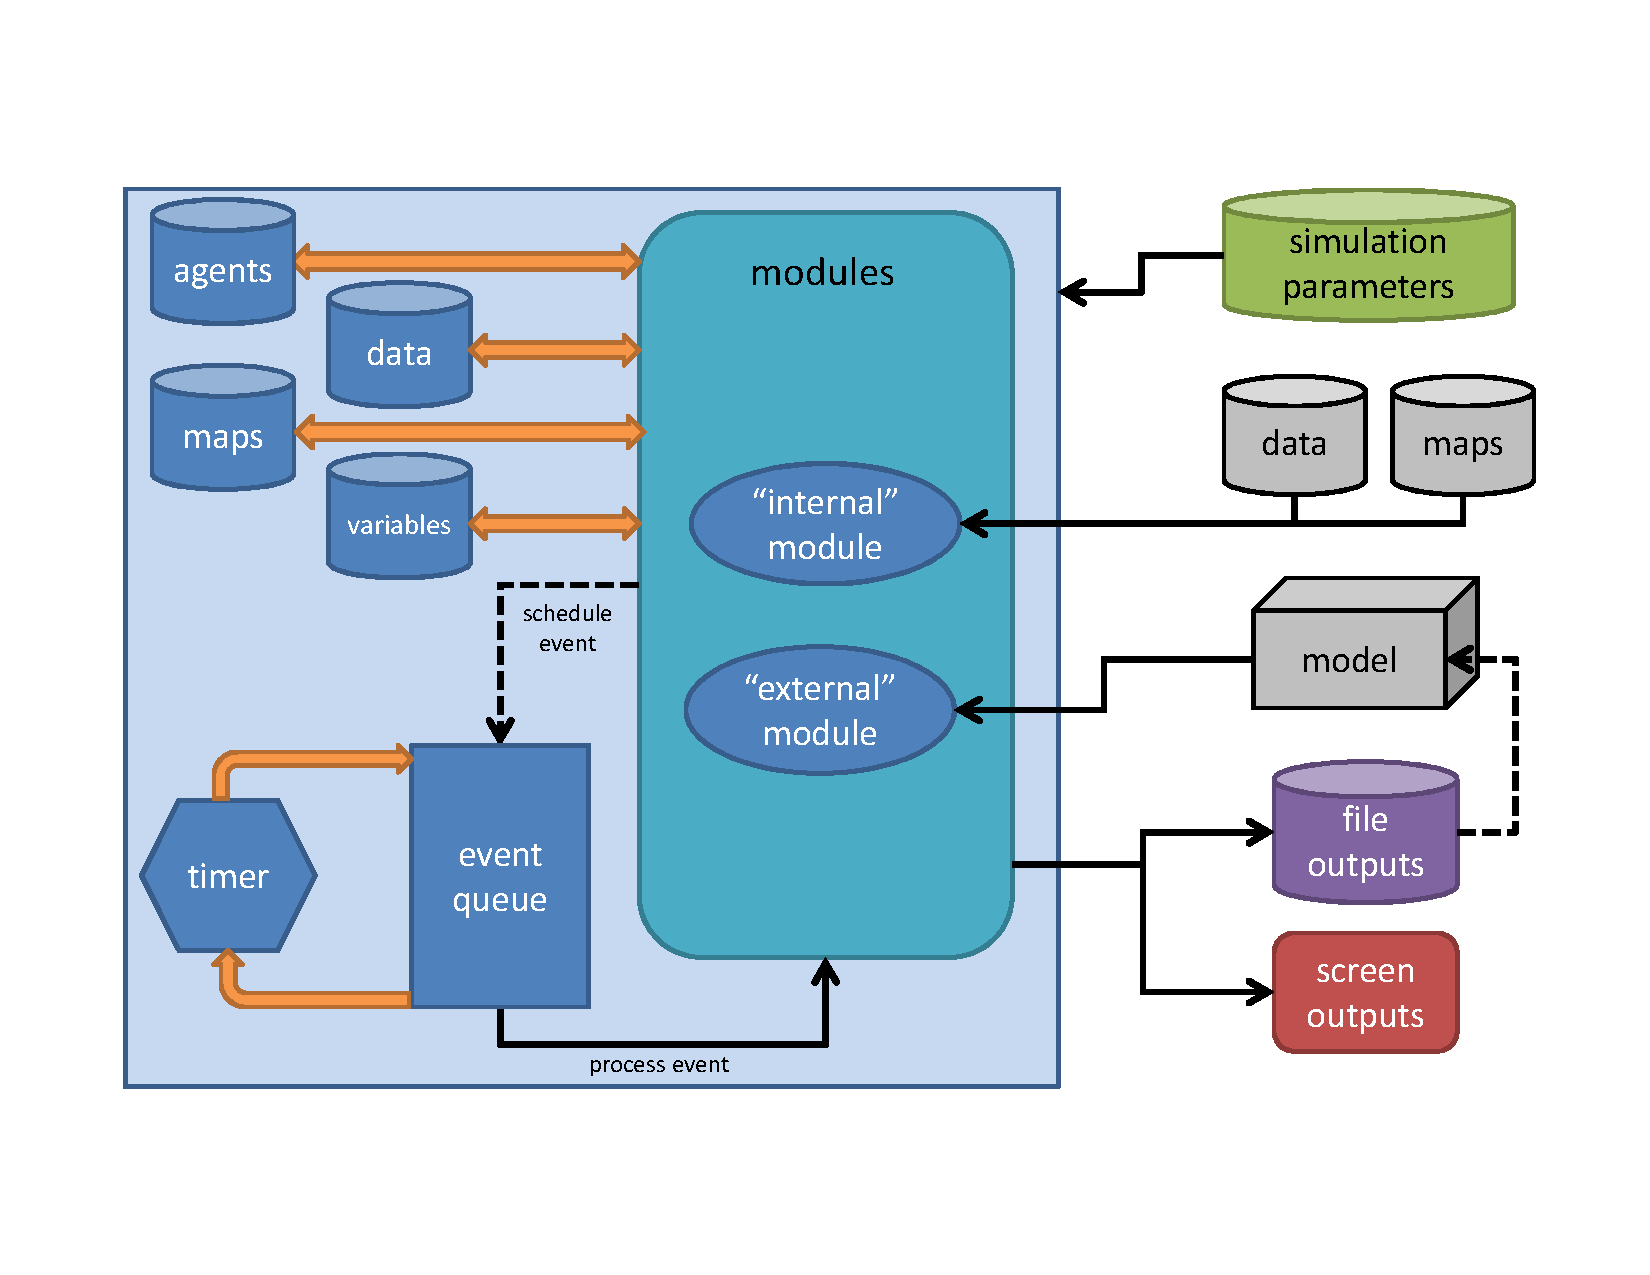
\includegraphics[width=5in]{../inst/SpaDES-overview-diagram.pdf}
	\caption{Schematic representation of a \texttt{SpaDES} simulation model.}
	\label{figure-SpaDES-overview}
\end{figure}

\subsection{\texttt{SpaDES} demos and sample modules}

\paragraph{}
The static nature of PDFs does not allow us to really show off the simulation visualization components of this package, so we invite you to check out the included demos, to run the sample simulation provided in this vignette, and to view the source code for the sample modules included in this package.

\subsubsection{Demos}

\begin{Schunk}
\begin{Sinput}
> library("SpaDES")
> # demo: randomLandscapes, fireSpread, caribouMovement
> demo("spades-simulation", package="SpaDES")
\end{Sinput}
\end{Schunk}

\newpage

\subsubsection{Sample model}

\begin{Schunk}
\begin{Sinput}
> library("SpaDES")
> outputPath=file.path("~", "tmp", "simOutputs")
> times <- list(start=0, stop=10.2)
> parameters <- list(.globals=list(.stackName="landscape", .outputPath=outputPath,
+                                  burnStats="nPixelsBurned"),
+                    .progress=list(NA),
+                    randomLandscapes=list(nx=1e2, ny=1e2, inRAM=TRUE),
+                    fireSpread=list(nFires= 1e1, spreadprob=0.225, its=1e6,
+                                    persistprob=0, returnInterval=10, startTime=0,
+                                   .plotInitialTime=0.1, .plotInterval=10),
+                    caribouMovement=list(N=1e2, moveInterval=1,
+                                         .plotInitialTime=1.01, .plotInterval=1)
+                    )
> modules <- list("randomLandscapes", "fireSpread", "caribouMovement")
> path <- system.file("sampleModules", package="SpaDES")
> mySim <- simInit(times=times, params=parameters, modules=modules, path=path)
> #dev(4)
> spades(mySim)
\end{Sinput}
\end{Schunk}
\includegraphics{introduction-using-SpaDES}

\newpage

\section{Using \texttt{SpaDES} to build simulations}

\paragraph{Requirements}
This packages makes heavy use of the \texttt{raster} and \texttt{sp} packages, so familiarity with these packages, their classes and methods is recommended. Plotting features are built using the \texttt{grid} package.

\subsection{Setting up a simulation:}
As you can see in the sample simulation code provided above, setting up and running a simulation in \texttt{SpaDES} is straightforward using existing modules. You need to specify somethings about the simulation environment including 1) all parameter values passed to the simulation, 2) which modules to use for the sim, and 3) any global data objects that should be used to store the simulation state. Each of these are passed as named lists to the simulation object upon initilization.

\paragraph{Initializing a simulation:}
The details of each simulation are stored in an S4 \texttt{simList} object, including the simulation parameters and modules used, as well as storing the current state of the simulation and the future event queue. A list of all completed events is also stored, which can provide useful debugging information.

\paragraph{}
A new simulation is initialized using the \texttt{simInit} function, which does all the work of creating the \texttt{simList} object for your simulation, setting all the slot values appropriately. Furthermore, this function tries to provide additional feedback to the user regarding parameters that may be improperly specified.

\paragraph{}
You can inspect the contents of a \texttt{simList} object as you would any other \textsf{R} object (\textit{e.g.}, \texttt{show(mySim)}).

\subsection{Running a simulation:}
Once a simulation is properly initialized it is executed using the \texttt{spades} function. By default, a progress bar is displayed in the console (this can be customized), and any specified files are loaded (via including a fileList dataframe, see examples). Debugging mode (setting \texttt{spades(mySim, debug=TRUE)}) prints the contents of the \texttt{simList} object after the completion of every event during simulation.

\newpage

\section{SpaDES modules}

\paragraph{}
\texttt{SpaDES} modules are event-driven, meaning that different actions are performed on data objects based on the order of scheduled events. A module describes the processes or activities that drive simulation state changes. Each activity consists of a collection of events which are scheduled depending on the rules of the simulation. Each event may evaluate or modify a simulation data object, or perform other operations such as saving and loading data objects or plotting.

\paragraph{}
The power of \texttt{SpaDES} is in modularity and the ease with which existing modules can be modified and new modules created. This vignette will highlight general use of the package and its features using the sample modules provided. Creating and customizing modules is a whole topic unto itself, and for that reason we have created a separate \texttt{modules} vignette with more details on module development.

\section{Simulation and data}

\paragraph{}
Historically, simulation models were built separately from the analysis of input data (\textit{e.g.}, via regression) and outputs of data (\textit{e.g.}, graphically, statistically). On the input data side, this effectively broke the linkage between data (\textit{e.g.}, from field or satellites) and the simulation. This has the undesired effect of creating the appearance of reduced uncertainty in simulation model predictions, by breaking correlations between parameter estimates (that invariably occur in analyses of real data). Conversely, on the data output side, numerous tools, such as optimization (\textit{e.g.}, pattern oriented modeling) or statistical analyses could not directly interact with the simulation model, unless a specific extension was built for that purpose. In R, those tools already exist and are robust. Thus, validation, calibration, and verification of simulation models can become rolled into the simulation model itself. This enhances transparency and reproducibility, both desired properties for scientific studies.

\paragraph{}
Bringing data into\textsf{R}is easy, and can be done using any of the built in data import tools. To facilitate this, we have provided additional functionality to easily load maps or data from files via the load module. To automatically import a list of files, simply provide it as a parameter named \texttt{.loadFileList} when initializing the simulation. See \texttt{?loadFiles} and the modules vignette for more information on the load module.

\begin{Schunk}
\begin{Sinput}
> ### Example: loading habitat maps
> 
> # use all built-in maps from the SpaDES package
> pathToMaps <- file.path(find.package("SpaDES", quiet=FALSE), "maps")
> fileList <- data.frame(files=dir(pathToMaps, full.names=TRUE, pattern= "tif"),
+                       functions="rasterToMemory", packages="SpaDES",
+                       stringsAsFactors=FALSE)
> # this list can be passed to simInit() as an entry in the parameter list
> mySim <- simInit(times=list(start=0.0, stop=10),
+                  params=list(
+                    .loadFileList=fileList,
+                    .progress=list(NA),
+                    .globals=list(.stackName="landscape", burnStats="nPixelsBurned"),
+                    #.globals=list(burnStats="nPixelsBurned"),
+                    fireSpread=list(nFires=1e1, spreadprob=0.225, persistprob=0,
+                                    its=1e6,returnInterval=10, startTime=0.1,
+                                    .plotInitialTime = 0, .plotInterval=10)
+                  ),
+                  modules=list("fireSpread"),
+                  path=system.file("sampleModules", package="SpaDES"))
> spades(mySim)
\end{Sinput}
\end{Schunk}
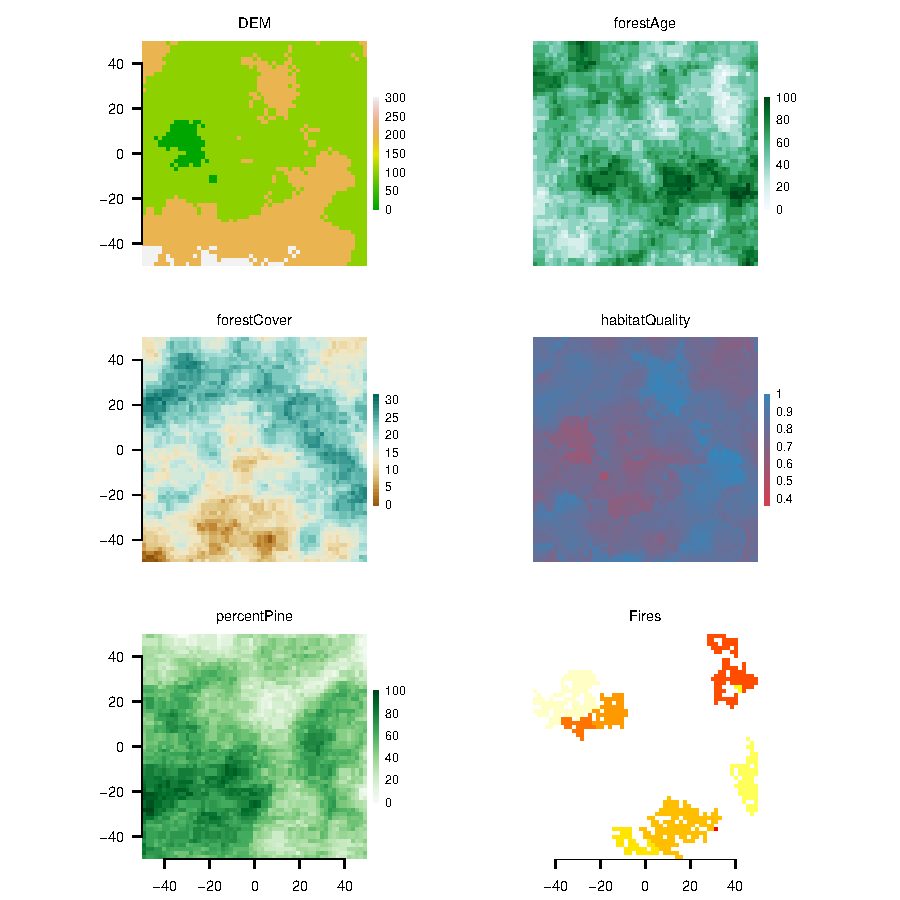
\includegraphics{introduction-load-landscape-maps}

\newpage

\section{Modelling spread processes}

\subsection{A simple fire model}

Using the \texttt{spread} function, we can simulate fires, and subsequent changes to the various map layers. Here, \texttt{spreadProb} can be a single probability or a raster map where each pixel has a probability. In the example below, each cell's probability is taken from the Percent Pine map layer.

\begin{Schunk}
\begin{Sinput}
> library(RColorBrewer)
> nFires <- 10
> landscape[["Fires"]] <-
+   spread(landscape[["percentPine"]],
+          loci=as.integer(sample(1:ncell(landscape), nFires)),
+          spreadProb=landscape[["percentPine"]]/(maxValue(landscape[["percentPine"]])*5)+0.1,
+          persistance=0,
+          mask=NULL,
+          maxSize=1e8,
+          directions=8,
+          iterations=1e6,
+          plot.it=FALSE,
+          mapID=TRUE)
> setColors(landscape$Fires)<-paste(c("#000000",brewer.pal(8,"Reds")[5:8]),c("00",rep("FF",4)),sep="")
> Plot(landscape[["Fires"]], add=FALSE)
\end{Sinput}
\end{Schunk}
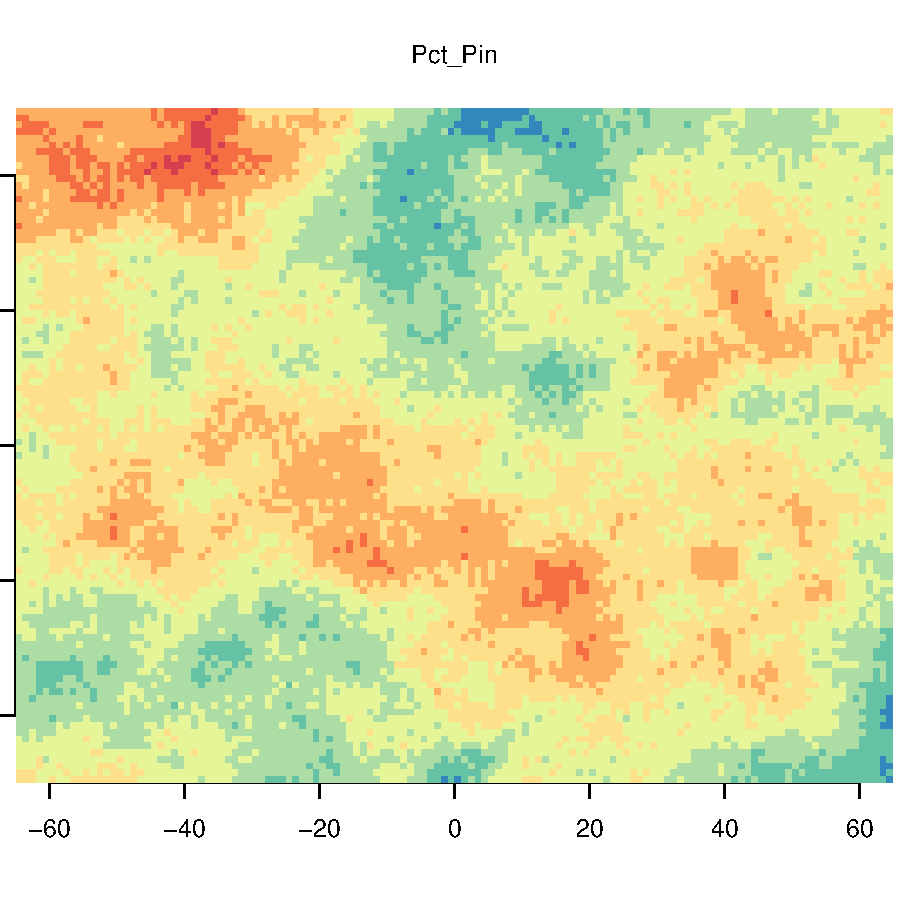
\includegraphics{introduction-fire}


\begin{Schunk}
\begin{Sinput}
> # Show the burning more strongly over abundant pine
> percentPine<-landscape$percentPine
> Plot(percentPine, add=FALSE)
> #Plot(landscape[["Fires"]], add=TRUE)
> Plot(landscape[["Fires"]], addTo="percentPine", legend=FALSE, title=FALSE)
\end{Sinput}
\end{Schunk}
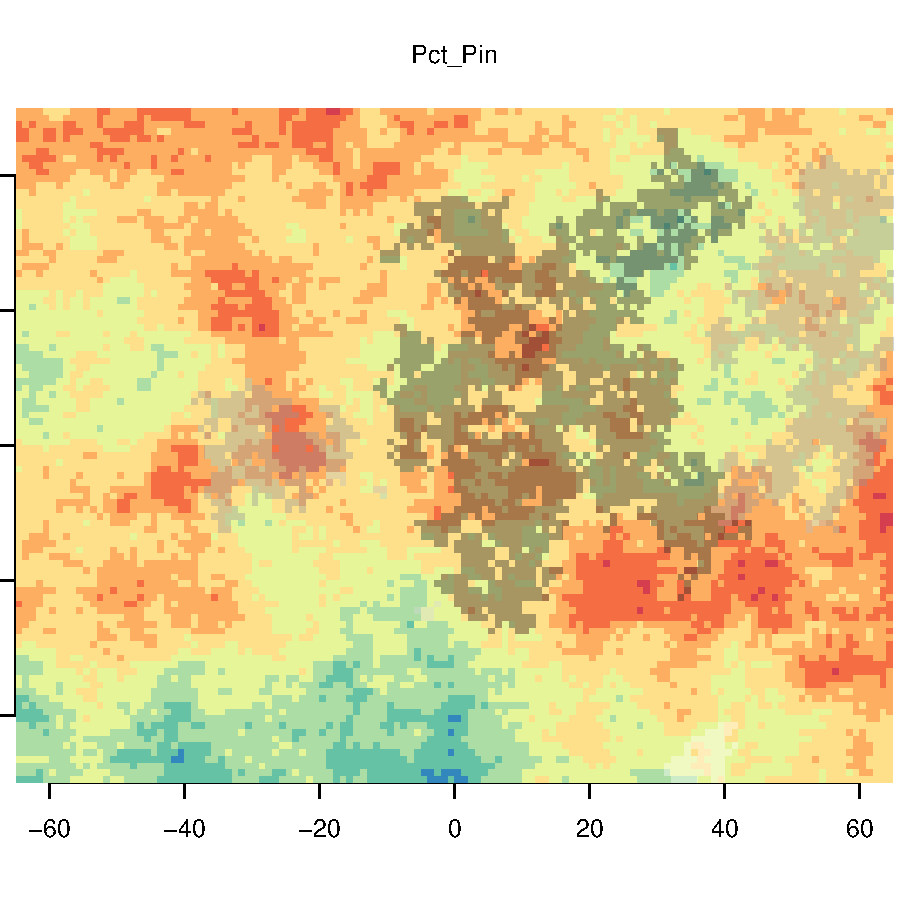
\includegraphics{introduction-fire-overlaid}

\paragraph{}
We can see that the fires tend to be in the Pines because we made it that way, using an arbitrary weighting with pine abundance:

\begin{Schunk}
\begin{Sinput}
> # Show the burning more strongly over abundant pine
> fire <- reclassify(landscape[["Fires"]], rcl=cbind(0:1, c(0,ncell(landscape)), 0:1))
> pine <- reclassify(landscape[["percentPine"]], rcl=cbind(0:9*10, 1:10*10, 0:9))
> PineByFire <- crosstab(fire, pine, long=TRUE)
> colnames(PineByFire) <- c("fire", "pine", "freq")
> PineByFire$pine <- as.numeric(as.character(PineByFire$pine))
> summary(glm(freq ~ fire*pine, data=PineByFire, family="poisson"))
\end{Sinput}
\begin{Soutput}
Call:
glm(formula = freq ~ fire * pine, family = "poisson", data = PineByFire)

Deviance Residuals: 
    Min       1Q   Median       3Q      Max  
-38.524  -15.008   -2.338   10.382   32.495  

Coefficients:
             Estimate Std. Error z value Pr(>|z|)    
(Intercept)  6.933599   0.019436  356.75   <2e-16 ***
fire1       -2.477138   0.070350  -35.21   <2e-16 ***
pine        -0.064018   0.003977  -16.10   <2e-16 ***
fire1:pine   0.255776   0.010681   23.95   <2e-16 ***
---
Signif. codes:  0 '***' 0.001 '**' 0.01 '*' 0.05 '.' 0.1 ' ' 1

(Dispersion parameter for poisson family taken to be 1)

    Null deviance: 9599  on 17  degrees of freedom
Residual deviance: 6691  on 14  degrees of freedom
AIC: 6829.8

Number of Fisher Scoring iterations: 5
\end{Soutput}
\end{Schunk}

\paragraph{}
Sure enough, there are more fires as the abundance of pine goes up, as seen by the positive interaction term (the negative \texttt{fire1} term means that there are more pixels without fires than with fires).

\paragraph{Impact some of the forest}
\begin{Schunk}
\begin{Sinput}
> landscape[["forestAge"]][landscape[["Fires"]]>0] <- 0
> landscape[["forestCover"]][landscape[["Fires"]]>0] <- 0
> landscape[["habitatQuality"]][landscape[["Fires"]]>0] <- 0.1
> landscape[["percentPine"]][landscape[["Fires"]]>0] <- 0
> Plot(landscape, add=FALSE)
\end{Sinput}
\end{Schunk}
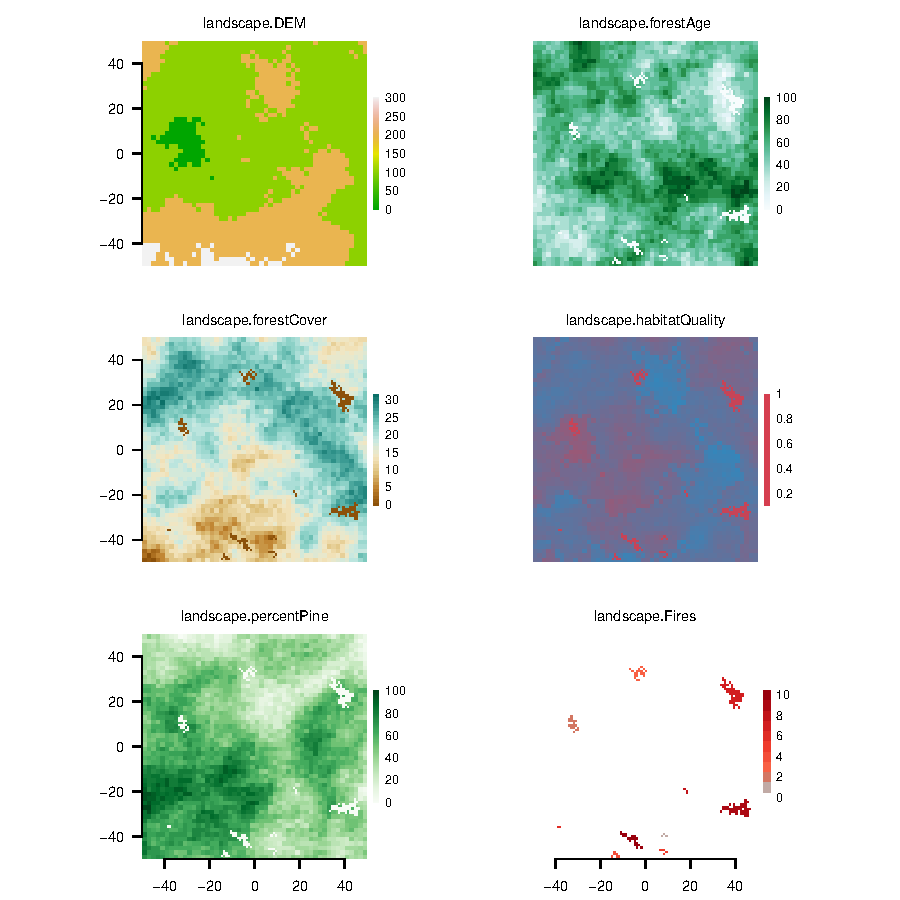
\includegraphics{introduction-fire-impacts-maps}

\newpage

\section{Agent based modelling}
A primary goal of developing \texttt{SpaDES} was to facilitate the development of agent-based models (ABMs), also known as individual-based models (IBMs).

\subsection{Point agents}

\paragraph{}
As ecologists, we are usually concerned with modelling individuals (agents) in time and space, and whose spatial location (position) can be represented as a single point on a map. These types of agents can easily be represented most simply by a single set of coordinates indicating their current position, and can simulated using a \texttt{SpatialPoints} object. Additionally, a \texttt{SpatialPointsDataFrame} can be used, which provides storage of additional information beyond agents' coordinates as needed.

\paragraph{}
These objects need to be named to work properly with SpaDES plotting, so you need to used the \texttt{SpatialPoint*Named} classes, which is easily done using \texttt{name}. This converts a \texttt{SpatialPoints*} object to its equivalent \texttt{SpatialPoint*Named}.

\paragraph{}
To model mobile point agents, \textit{e.g.}, animals (as opposed to non-mobile agents such as plants), use a \texttt{SpatialPointsDataFrameNamed} containing additional columns for storing agents' previous \texttt{n} positions.

\begin{Schunk}
\begin{Sinput}
> N <- 10 # number of agents
> # caribou data vectors
> IDs <- letters[1:N]
> sex <- sample(c("female", "male"), N, replace=TRUE)
> age <- round(rnorm(N, mean=8, sd=3))
> x1 <- runif(N, -50, 50) # previous X location
> y1 <- runif(N, -50, 50) # previous Y location
> # caribou (current) coordinates
> x0 <- rnorm(N, x1, 5)
> y0 <- rnorm(N, y1, 5)
> # create the caribou agent object
> # caribou needs to be a named object for plotting, use SpatialPointsDataFrameNamed
> caribou <- SpatialPointsDataFrameNamed(coords=cbind(x=x0, y=y0),
+                                   data=data.frame(x1, y1, sex, age),name="caribou")
> row.names(caribou) <- IDs
> 
\end{Sinput}
\end{Schunk}

\paragraph{}
Using a simple landscape-dependent correlated random walk, we simulate the movement of caribou across a heterogeneous landscape. Because we had just had fires, and we assume that fires have a detrimental effect on animal movement, we can see the long steps taken in the new, low quality, post-burn sections of the landscape.

\begin{Schunk}
\begin{Sinput}
> #dev(4)
> Plot(landscape[["habitatQuality"]], add=FALSE)
> for (t in 1:10) {
+   #crop any caribou that went off maps
+   caribou <<- crop(caribou,landscape)
+   drawArrows(from=SpatialPoints(cbind(x=caribou$x1, y=caribou$y1)),
+              to=caribou, length=0.04, addTo="habitatQuality")
+ 
+   # find out what pixels the individuals are on now
+   ex <- landscape[["habitatQuality"]][caribou]
+ 
+   #step length is a function of current cell's landscape quality
+   sl <- 0.25/ex
+ 
+   ln <- rlnorm(length(ex), sl, 0.02) # log normal step length
+   sd <- 30 # could be specified globally in params
+ 
+   caribou <<- crw(caribou, stepLength=ln, stddev=sd, lonlat=FALSE)
+ }
\end{Sinput}
\end{Schunk}
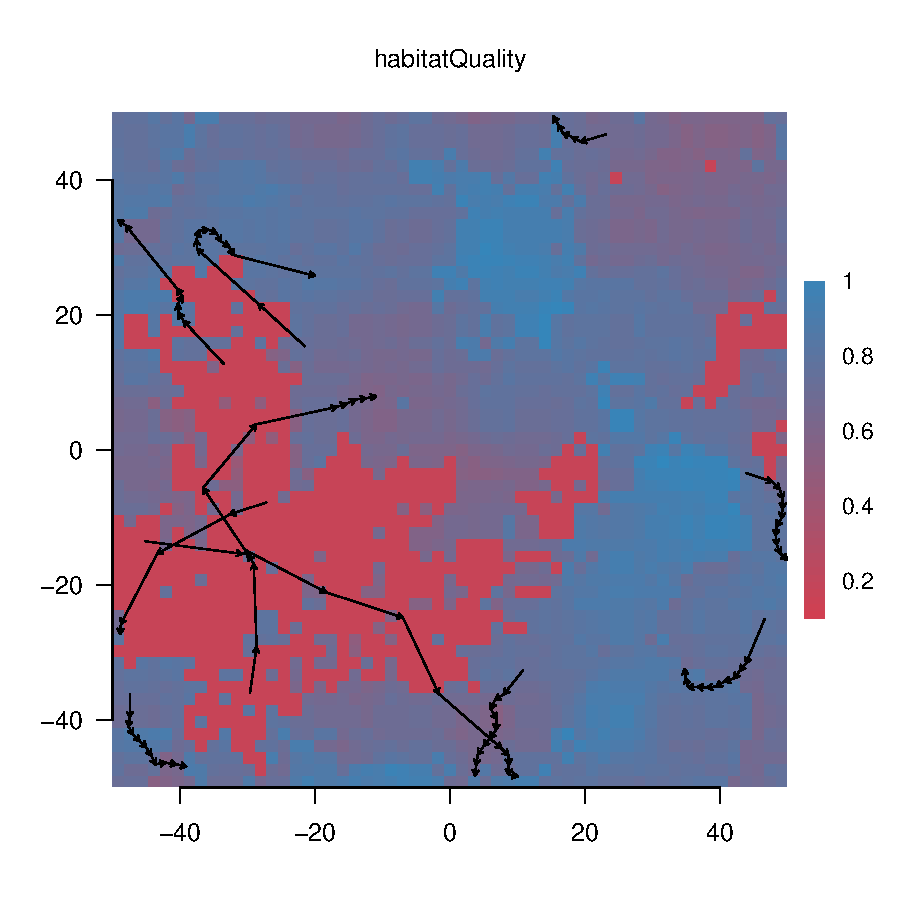
\includegraphics{introduction-agent-crw-trajectory}

\subsubsection{Polygons agents}

\paragraph{}
Analogously, it is possible to use \texttt{SpatialPolygons*}, but we haven't built \texttt{Plot} plotting methods for these yet.

\newpage

\section{Putting it all together}

\paragraph{}
Running multiple simulations with different parameter values is a critical part of sensitivity analysis, simulation experiments, optimization, and pattern oriented modelling. Below is a greatly simplified example, using the sample \texttt{randomLandscapes} and \texttt{fireSpread} modules. \textit{NB only two parameters are varied; no outputs are saved; and the analyses done here are kept simple for illustrative purposes. This will take a while to run!}

\begin{Schunk}
\begin{Sinput}
> ### WARNING this can take a while to run, especially for large mapSizes.
> 
> rasterOptions(maxmemory=1e9)
> # list all parameter values to run sims with
> parameters <- list(mapSize=round(sqrt(c(1e4, 1e5, 1e6, 1e7, 1e8))),
+                    pSpread=seq(0.05, 0.25, 0.05))
> # create data.frame with all parameter combinations
> paramsdf <- expand.grid(parameters)
> # outputs
> nPixelsBurned <- numeric()
> meanPixelsBurned <- cbind(paramsdf, pmean=NA, psd=NA)
> set.seed(42)
> for (i in 1:nrow(paramsdf)) {
+   # initialize each simulation with a param combo from paramsdf
+   mySim <- with(paramsdf,
+                 simInit(times=list(start=0.0, stop=20.0),
+                         params=list(
+                           .progress=list(.graphical=NA, .progressInterval=NA),
+                           .globals=list(.stackName="landscape", burnStats="nPixelsBurned"),
+                           randomLandscapes=list(nx=mapSize[i], ny=mapSize[i],
+                                                 inRAM=TRUE),
+                           fireSpread=list(nFires=1000, spreadprob=pSpread[i],
+                                           persistprob=0, its=1e6,
+                                           returnInterval=10, startTime=0)
+                           ),
+                         modules=list("randomLandscapes", "fireSpread"),
+                         path=system.file("sampleModules", package="SpaDES")))
+   mySim <- spades(mySim)
+ 
+   # collect stats for each run
+   proportionBurned <- with(paramsdf, nPixelsBurned / (mapSize[i]^2))
+   meanPixelsBurned[i, "pmean"] <- mean(proportionBurned)
+   meanPixelsBurned[i, "psd"] <- sd(proportionBurned)
+ 
+   # cleanup between runs
+   rm(landscape, mySim, nPixelsBurned)
+   for (j in 1:10) gc()
+ }
> # overall statistics
> pch <- c(21:25)
> col <- brewer.pal(5, "Set1")
> with(meanPixelsBurned, plot(pmean ~ pSpread, xlab="Spread probability",
+                             ylab="Mean proportion of pixels burned",
+                             ylim=c(0,1), pch=pch, cex=1.5, col=col))
> with(parameters, legend("topleft", legend=formatC(mapSize^2, digits=0),
+                               pch=pch, col=col, cex=1.2))
\end{Sinput}
\end{Schunk}


\begin{figure}[!htbp]
  \centering
  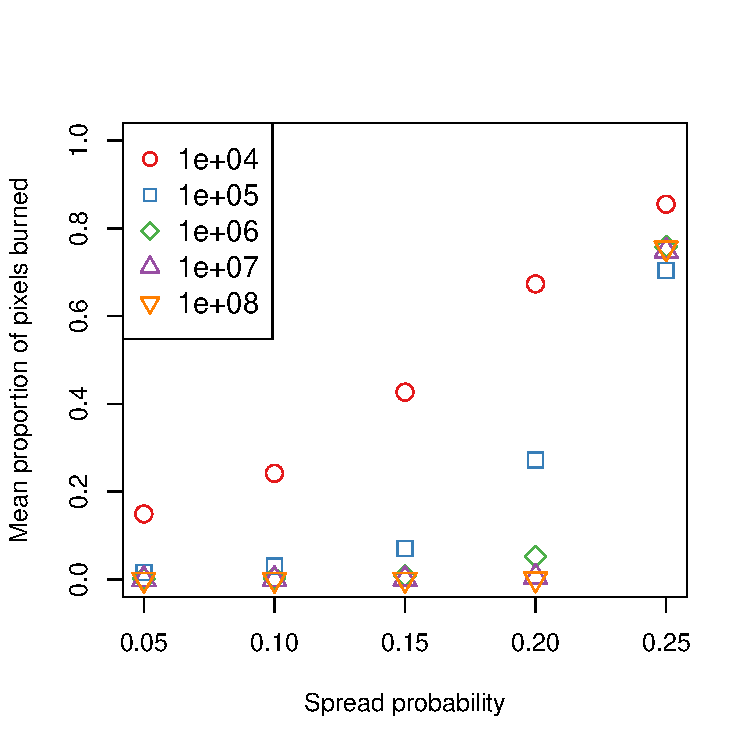
\includegraphics[width=5in]{../inst/plot-area-burned.pdf}
	\caption{Mean proportion of pixels burned for maps of various sizes and fire spread probabilities.}
	\label{figure-area-burned}
\end{figure}

\newpage

\section{Additonal resources}

\subsection{\texttt{SpaDES} documentation and vignettes}

\paragraph{Vignettes:}

\begin{itemize}
  \item \texttt{introduction}: Introduction to SpaDES: A package to develop and run spatially explicit discrete event simulation models. [This vignette.]
  \item \texttt{modules}: Building modules in \texttt{SpaDES}.
  \item \texttt{plotting}: Plotting with \texttt{SpaDES}.
  \item \texttt{debugging}: Debugging simulations built using \texttt{SpaDES}. [Not yet written.]
\end{itemize}

\subsection{Reporting bugs}

\paragraph{}
As with any software, there are likely to be issues. If you believe you have found a bug, please contact us via the package GitHub site: \url{https://github.com/achubaty/SpaDES/issues}. Please do not use the issue tracker for general help requests. We will soon be setting up a help mailing list soon for users who seek assistance using \texttt{SpaDES}.

\end{document}
